\documentclass[../manuscript]{subfiles}
\def\biblio{\bibliographystyle{plainnat}\bibliography{bibliography}}
\usepackage{Sweave}
\begin{document}


\section[Experiment 3]{Experiment 3. Robustness of scaling to stimulus properties.}
\label{sec:grid}

We have characterized the interference between moving elements in the
display leading to reversal of percieved motion in terms of their
spatial separation, and have observed that the critical spacing at
which opposing local motion interferes with global motion appears to
scale proportionately to eccentricity. However, the size and
speed of the elements in our display were also scaled proportionate to their
eccentricity. This leaves open an alternate explanation in which the
motion reversal is dependent on the distance between the objects
\emph{relative} to their size of the objects, Under this hypothesis,
the critical spacing might be better described in units of a multiple
of the size of the envelope, or the period of the grating, rather than
the separation between centers. For example, contour integration among Gabor patches has been characterized as a function of the ratio of inter-element spacing to envelope size \citep{Beaudot:2003dz} In this section, we vary the size the motion
elements, as well as their local and global speeds, and measure what effects these
parameters have on the critical distance.

A second motivation is to solidify the connection between our motion
stimulus and the phemonenon of crowding. As we have seen the
scaling of critical distance with spacing in our display is similar to
that observed for crowding. A noted property of crowding in parafoveal vision is that the the range of
spatial interaction is not strongly dependent on the size of the
target or the flankers \citep{Levi:2002cs,Tripathy:2002kx}; this has
been proposed as a diagnostic test for crowding as opposed to other
kinds of suppressive spatial interaction \citep{Pelli:2004km}. If motion 
integration is subject to the same effects of crowding as other forms of spatial
feature integration, it may reflect a common computational principle
or even a shared neural mechanism underlying such processes. \todo{Last sentence probably belongs in Discussion.}

\subsection{Methods}
\label{sec:grid_methods}

Subjects repeated the direction discrimination task, with the same
basic structure and equal proportion of congruent, incongruent and
counterphase stimuli as in previous sections. As in
\autoref{occlusion} we used the QUEST procedure to select the target
density (expressed as the number of targets in the full circle) for
each trial. Within each session we varied one of the stimulus
parameters across three values, those being 66\%, 100\% and 150\% the
values used in \autoref{sec:constant}. Stimulus sizes were otherwise
scaled proportionate to eccentricity, as in
\autoref{sec:constant}. QUEST trials were interleaved across three
stimulus values and four eccentricity values, so that 12 QUEST
sequences were interleaved in each session. Data from
separate days were pooled.

\subsubsection{Stimulus variations and scaling}
\label{sec:stim-vari-scal}
We tested three variations of the
stimulus: temporal frequency, spatial period, and spatial step size
(\autoref{fig:grid-tableaux}). Since we leave the spatial bandwidth
parameter constant, lengthening the spatial period also lengthens the
envelope of the individual motion elements, and since the temporal
frequency is held constant, lengthening the period also increases the
speed of the local motion component of the stimulus. The second
manipulation is a change in temporal frequency of the stimulus. This
has the effect of changing the speed of the local motion component of
the stimulus, without changing its size or spatial frequency. The
third manipulation is a change in the step distance between each
appearance of the local element. This changes the speed of the global
translation, leaving local speed unchanged. 

\todo{I'm adding this. It will put the motion energy analysis on more
  solid ground.} A fourth manipulation is to directly manipulate the
balance of local motion energy content. We do this by superposing
conguent and incongruent local motion in the same
stimulus, in the same way that we constructed our counterphase stimulus by superposing congruent and incongruent local motion stimuli.  

\begin{figure}
  \begin{center}
    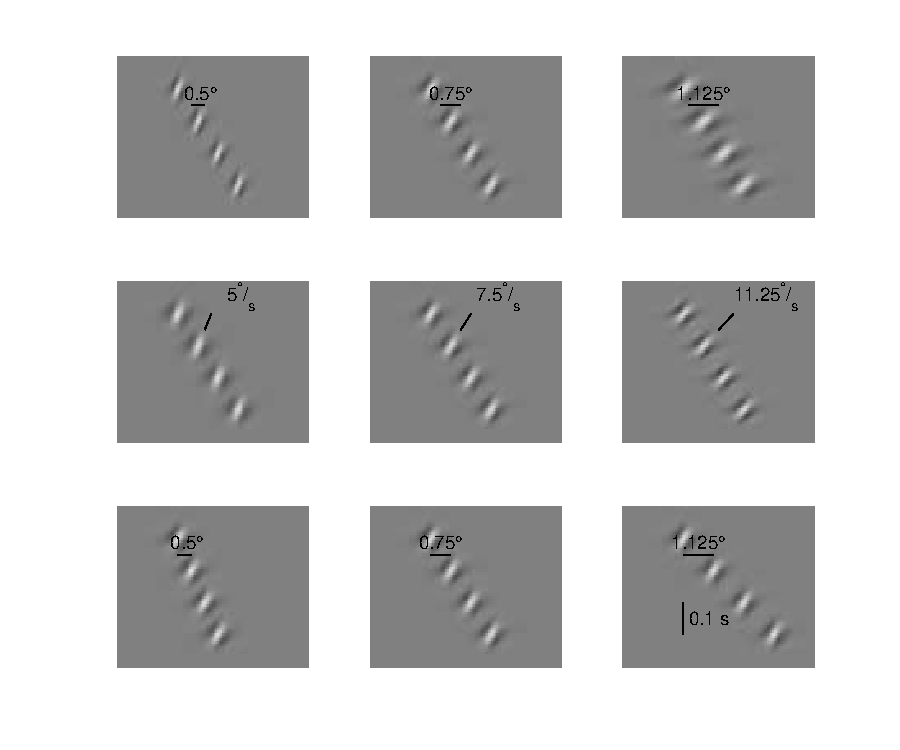
\includegraphics[width=.75\linewidth]{../grid_figure.pdf}
    \end{center}
    \caption{Stimulus manipulations. $(x,t)$ diagrams of the
      stimuli show the manipulations undertaken. Top row: the element
      size and spatial period increase from left to right. Middle row:
      The local speed and temporal frequency increase from left to
      right Bottom row: The step size increases from left
    to right. Stimuli in the middle column are identical. Note that
    the manipulations of element size and step size produce stimuli
    that are spatially compressed or elongated versions of each other.}
    \label{fig:grid-tableaux}
\end{figure}

\subsubsection{Motion energy analysis.}
\label{sec:grid-motion-energy-methods}

For each unique configuration of the stimulus values, up to a rotation, we calculated the luminance values along the circle passing through the element centers, sampled at the monitor frame rate. To this data we applied a motion-energy model, similar to \cite{Adelson:1985ea}, using space-time separable anaysis filters. The spatial analysis filters were intended to approximate the bandpass properties of direction selective channels in human vision; to that extent we used a set of Cauchy filters \citep{Klein:1985rz} with the center frequencies matched to those of the stimuli. The spatial bandwidth of the filters was dependent on the center frequency and the eccentricity, consistent with the bandpass properties inferred from human psychophysics; in particular, at a given eccentricity, the bandwidths of the filters decrease with increasing spatial frequency \todo{I suppose it's not ``bandwidth" but Q-factor of the filter. The filter width contains more oscillations at higher frequencies is the main point.} \citep{Anderson:1987oq,Banks:1991kl,Anderson:1991tg}. The bandwidths chosen for the analysis filters were thus a function of both eccentricity and center spatial frequency; we selected the spatial extent of each anaysis filter by interpolating the measurements of \citet{Banks:1991kl}. The parameters used at each eccentricity are given in \autoref{table:motion_energy}. On the other hand, the temporal component of each filter was identical at all cases, because temporal sensitivity does not appear to vary with spatial frequency or eccentricity \citep{Virsu:1982fv,Wright:1983dz}. The temporal component of each filter was the same as used in \cite{Kiani:2008uq}.

\subsection{Results}
\label{sec:grid-results}

\begin{figure}
  \begin{center}
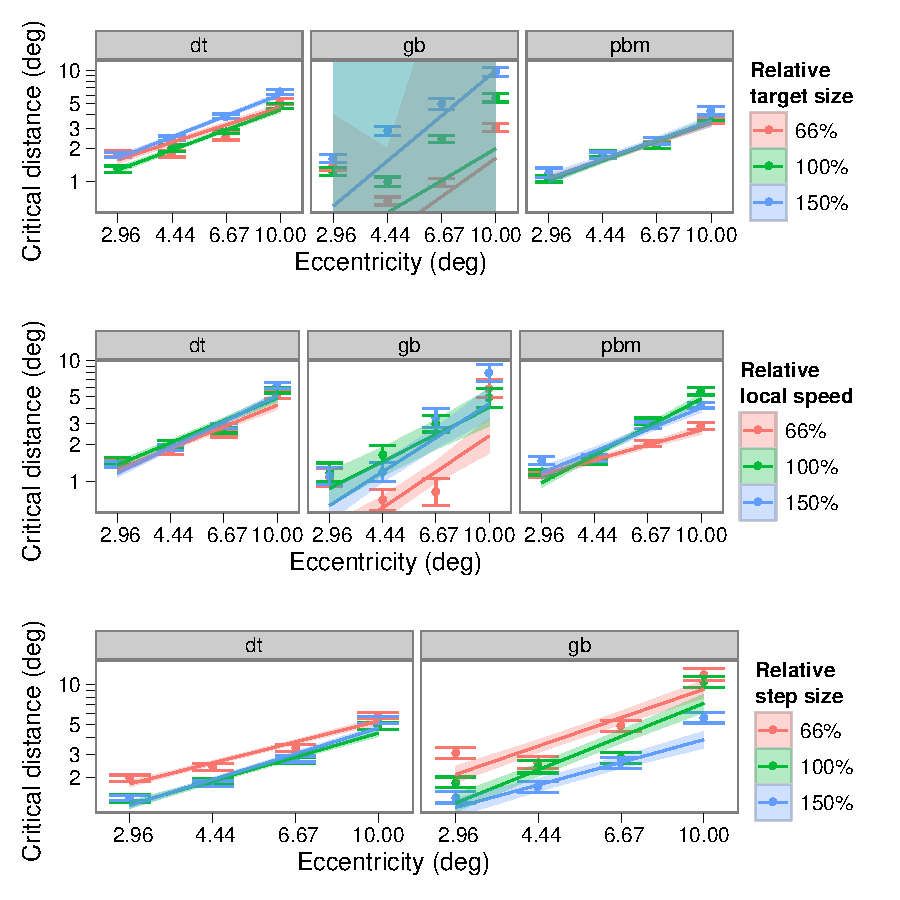
\includegraphics{figure_3-gridplot}
\end{center}
    \caption{Effect of stimulus on critical distance. Each plot
      shows critical distance for each subject, as a stimulus
      parameter is varied. Error bars show standard error of the
      measured critical distance at each condition. Lines show best
      fit to a power law for critical distance as a function of
      eccentricity; shaded region shows standard error on that
      fit. Rows correspond to rows in \autoref{fig:grid-tableaux};
      columns correspond to subjects; colors correspond to stimulus
      parameters (columns in \autoref{fig:grid-tableaux}.) Conditions
      where critical distance varies significantly as stimulus
      parameters change are labeled with $*$ ($p < 0.05$)
      }
    \label{fig:grid-scaling}
\end{figure}

\subsubsection{Element size}
\label{sec:spatial-frequency}

\todo{Ignore subject GB here. He can barely see the local motion
  (misses a lot of \emph{congruent} catch trials at high density.)
  Looking at his data did convince me to start thinking about the
  balance of global motion discriminability and local motion energy. But I don't think i
  can use his data.}

In the first row of \autoref{fig:grid-scaling} we see that the approximately proportional relation of stimulus size to critical distance is maintained at the target size is enlarged or shrunk. There is no significant change in the shape of this slope, however there may be a small enlargement of the critical spacing as the target size is increased. Note that the absolute stimulus size still scaleswith eccentricity in this experiment; the stimulus size is adjusted relative to the baseline of sizes used in \autoref{sec:constant}. In the first row of \autoref{fig:grid-physical} we plot the critical distance as a function of the absolute stimulus size. This allows us to see that while holding element size constant over a range of eccentricities, that critical spacing still scales with eccentricity. \todo{Again ignoring GB. But it's interesting that GB collapses into size-determined behavior when he can't see the local motion.} The small shift of critical distance with target size is on the same order as the element size itself. This result is consistent with crowding because our critical distance has been measured from element center to element center. For large flankers, it is typically the edge-to-edge distance between target and flanker at critical spacing that is invariant to target size \citep{Levi:2002cs}. \todo{This also may touch on the question of the slope of the psychometric function. Do larger flankers result in different slopes? If so, then the particular threshold level I choose for "critical distance" affects the description of the data.}

\subsubsection{Local speed}
\label{sec:grid-temporal-frequency}

We then measured how critical distance changed as a function of the local speed, which was varied by changing the temporal frequency of phase rotation in each local motion element. The second rows of \autoref{fig:grid-scaling} shows that the scalar dependence of critical distance on eccentricity does not significantly change as local speed changes. This indicates to us that if the 

and \autoref{fig:grid-physical} show how the measurement of 

\subsubsection{Step size}
\label{sec:step-size}

We then changed the step size of the global translation of each element. We found that the critical separation actually decreased somewhat with increasing step size (\autoref{fig:grid-physical}, row 3). At first glance it is difficult to interpret this finding. The result is somewhat contrary to our intuitions; if
``misbinding'' were taking place between a the present instance of a target and a true future instance of a distractor, a larger step size would be seen to bring the flanker closer to the previous position of the true target and then lead to an increased critical spacing for increased step sizes. \todo{this speculation probably belongs in Discussion.} However it is not clear that this intuitive temporal structure (a local motion leading to an prediction of future position shift leading to a misbinding) reflects the true computation taking place. Before speculating too deeply on mechanism we must account for the changes in strength of the local motion signal and the global position-change signal. That is the subject of the next section.

\subsubsection{Strength of local and global motion in various stimuli.}
\label{sec:motion-energy}

The point can be regarded as the. While changing the flanker distance between widely spaced targets does not affect their local motion energy, crowding has been seen as a kind of equivalent of adding noise about the position of basic features. Thus the ability to detect. We see this in the one third of our trials that use ambiguous "counterphase" motion stimuli that 

While widely separated flankers do not appreciably affect the local motion energy of the stimuli, the interactions between successive appearances of the local motion elements do have an affect. When we change the size of the local motion elements, or the global step size, we affect the amount of spatial overlap between the successive elements. A local motion detector, such as a complex cell in area V1, whose receptive field is located between
the location of two successive presentations of a local element,
may be affected by the degree of overlap. It may also be affected by whether the successive elements have their peaks and troughs aligned so that they constructively or descructively interfere; all elements in our displays were presented in cosine phase, so out manipulations affect the alignment of peaks between successive elements. We performed a motion energy analysis as described in \autoref{sec:grid-motion-energy-methods}. \todo{An experiment titrating the amount of motion energy -- putting stimuli on a continuum between "incongruent" and "congruent" by varying the contrast of each -- will help me out here as well.}


\begin{figure}
  \begin{subfigure}[b]{\linewidth}
  \begin{center}
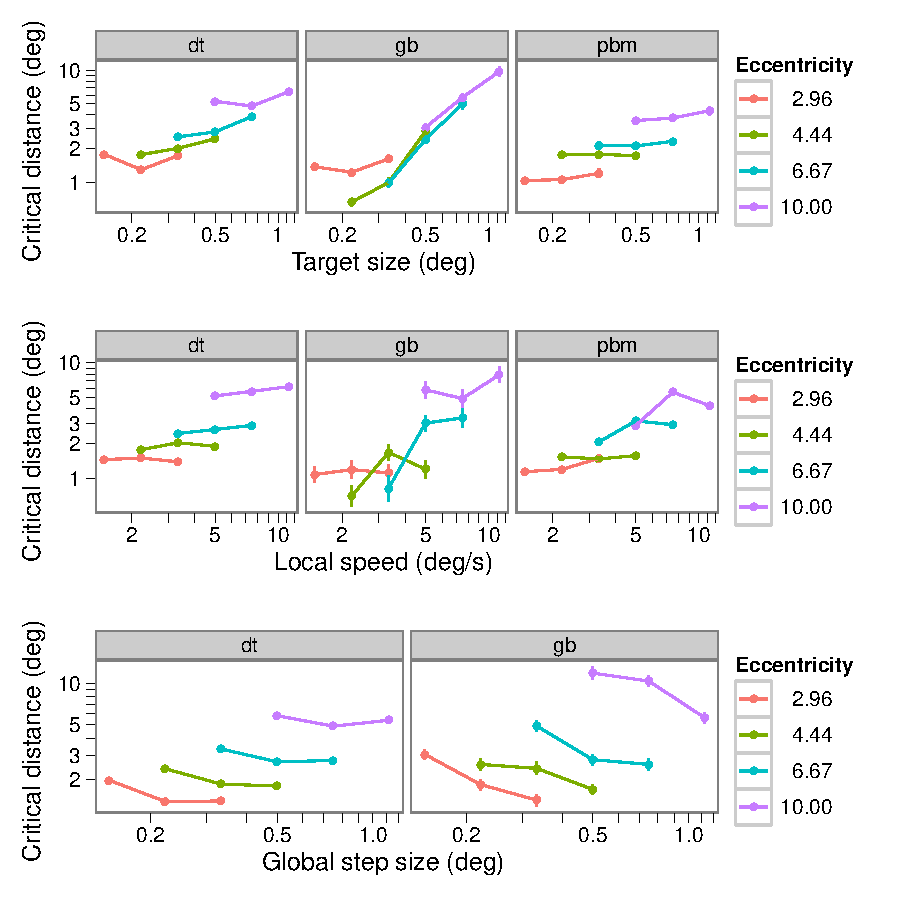
\includegraphics{figure_3-grid_physical}
\end{center}
    \subcaption{Critical distances from \autoref{fig:grid-scalng} are plotted again, with the horizontal coordinate being the physical size of the parameter being varied as indicated in \autoref{fig:grid-tableaux}. Rows correspond to rows in \autoref{fig:grid-tableaux}. \todo[inline]{I don't think the error bars ought to be this small; I blame the way that the slopes of the psychometric function have been fixed per-subject.} }
    \label{fig:grid-physical}
  \end{subfigure}
  \begin{subfigure}[b]{\linewidth}
    \missingfigure{Plot critical distance for SF data as ratio to stimulus size}
    \subcaption{For the experiment varying target size, critical distance is replotted as a multiple of the target size.}
    \label{fig:grid-relative}
  \end{subfigure}
  \caption{}
\end{figure}

\begin{figure}
	\begin{subfigure}[b]{\linewidth}
	  \missingfigure[figwidth=\linewidth]{x-t and spectrum of local, congruent, and global elements.}
	  \subcaption{Fourier spectra corresponding to local and global motion. Dotted outlines show the full width at half maximum of filters used in our motion energy analysis. Left shows the spectrum of a single element. Middle plot shows the spectrum of congruent motion. Right plot shows the spectrum of incongruent motion. Dotted outlines show the passband (full width at half maximum) of the analysis filters used to extract the motion energy.}
	  \label{fig:spectra}
	\end{subfigure}
	\begin{subfigure}[b]{\linewidth}
		\missingfigure{Motion energy for each stimulus used in \autoref{sec:grid}. Values range from -1 (all motion energy incongruent to global direction) to 1 (all motion energy congruent to ) }
	\end{subfigure}
	\caption{}
\end{figure}

\biblio
\end{document}
